\documentclass[12pt,letterpaper]{article}
\usepackage{graphicx,textcomp}
\usepackage{natbib}
\usepackage{setspace}
\usepackage{fullpage}
\usepackage{color}
\usepackage[reqno]{amsmath}
\usepackage{amsthm}
\usepackage{fancyvrb}
\usepackage{amssymb,enumerate}
\usepackage[all]{xy}
\usepackage{endnotes}
\usepackage{lscape}
\newtheorem{com}{Comment}
\usepackage{float}
\usepackage{hyperref}
\newtheorem{lem} {Lemma}
\newtheorem{prop}{Proposition}
\newtheorem{thm}{Theorem}
\newtheorem{defn}{Definition}
\newtheorem{cor}{Corollary}
\newtheorem{obs}{Observation}
\usepackage[compact]{titlesec}
\usepackage{dcolumn}
\usepackage{tikz}
\usetikzlibrary{arrows}
\usepackage{multirow}
\usepackage{subcaption}
\usepackage{xcolor}
\newcolumntype{.}{D{.}{.}{-1}}
\newcolumntype{d}[1]{D{.}{.}{#1}}
\definecolor{light-gray}{gray}{0.65}
\usepackage{url}
\usepackage{listings}
\usepackage{color}

\definecolor{codegreen}{rgb}{0,0.6,0}
\definecolor{codegray}{rgb}{0.5,0.5,0.5}
\definecolor{codepurple}{rgb}{0.58,0,0.82}
\definecolor{backcolour}{rgb}{0.95,0.95,0.92}

\lstdefinestyle{mystyle}{
	backgroundcolor=\color{backcolour},   
	commentstyle=\color{codegreen},
	keywordstyle=\color{magenta},
	numberstyle=\tiny\color{codegray},
	stringstyle=\color{codepurple},
	basicstyle=\footnotesize,
	breakatwhitespace=false,         
	breaklines=true,                 
	captionpos=b,                    
	keepspaces=true,                 
	numbers=left,                    
	numbersep=5pt,                  
	showspaces=false,                
	showstringspaces=false,
	showtabs=false,                  
	tabsize=2
}
\lstset{style=mystyle}
\newcommand{\Sref}[1]{Section~\ref{#1}}

\title{ Problem Set 1 Response}
\date{October 1st, 2022}
\author{Ariana Antunes}

\begin{document}
	\maketitle
	

\section*{Question 1 (50 points): Education}

\textit{1. 90% confidence interval for the average student IQ in the school.}\\

\vspace{.25cm}

\lstinputlisting[language=R, firstline=56, lastline=68]{AA_PS01.R}  
\vspace{.25cm}

\begin{verbatim}
	    Lower    Upper 
	    94.13283 102.7472
	    
	    mean(y)[1] 98.44

\end{verbatim}

\textit {2. Next, the school counselor was curious whether the average student IQ in her school is higher than the average IQ score (100) among all the schools in the country.
Using the same sample, conduct the appropriate hypothesis test with α = 0.05.} \\

\lstinputlisting[language=R, firstline=80, lastline=85]{AA_PS01.R}  
\vspace{.25cm}

\begin{verbatim}
	One Sample t-test 
	
	data: y
	t = 37.593, df = 24, p-value < 2.2e-16
	alternative hypothesis: true mean is not equal to 0
	
	5 percent confidence interval: 98.27407 98.60593
	sample estimates:mean of x     
	98.44 
	
\end{verbatim}
\vspace{.5cm}

\section{Question 2 (50 points): Political Economy}

\subsection*{The correlation plot between Y, X1, X2 and X3} 

\noindent You can also save figures in R, and place them in your answers that you're writing in your .tex file. First, you need to make sure your path/file name is correct, then you'll save your work when your in R (see code below).

\lstinputlisting[language=R, firstline=118, lastline=119]{AA_PS01.R}  
\vspace{.25cm}
\noindent With our figure saved, we just need to render it in our .tex file, which we can do using the \texttt{figure} environment:


\begin{figure}[h!]\centering
	\caption{\footnotesize Correlation between Y, X1, X2 and X3.}
	\label{fig:plot_1}
	\includegraphics[width=.75\textwidth]{correlation_expenditure_plot.png}
\end{figure}

It seems the correlation appears to be much similar when compering the different variables. 

\subsection*{The correlation plot between Y and Region}


\begin{figure}[h!]\centering
	\caption{\footnotesize correlation plot  between Y and Region.}
	\label{fig:plot_1}
	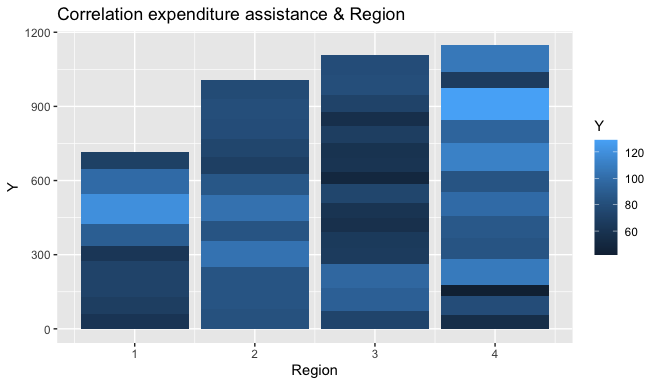
\includegraphics[width=.75\textwidth]{plot_Y+Region.png}
\end{figure}

On average west region have the highest per capita expenditure on housing assistance. 


\subsection*{The correlation plot between Y, X1 and Region}


\lstinputlisting[language=R, firstline=137, lastline=139]{AA_PS01.R}  


\begin{figure}[h!]\centering
	\caption{\footnotesize correlation plot  between Y and Region.}
	\label{fig:plot_1}
	\includegraphics[width=.75\textwidth]{CorrelationYX1&Region.png}
\end{figure}



\end{document}
